\documentclass[tikz,border=3pt]{standalone}
\usepackage{amsmath,bm,xcolor}
\usetikzlibrary{arrows.meta}
\begin{document}
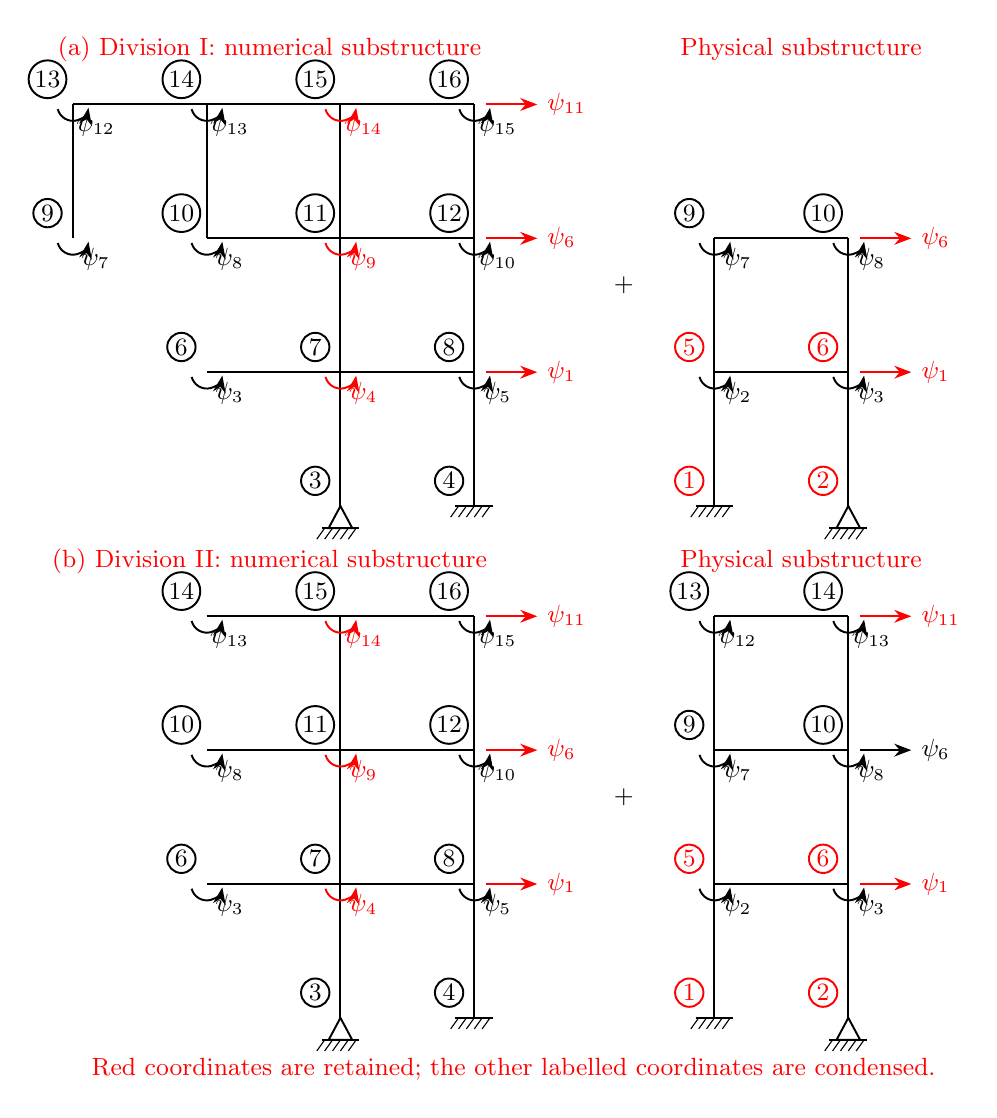
\begin{tikzpicture}[>=Stealth,every node/.style={font=\fontsize{9}{11}\selectfont},line width=.7pt]
\begin{scope}[shift={(0,6.5)}]
\draw[] (3.4,0)--(3.4,5.1);
\draw[black] (3.4,0)--(3.25,-0.28)--(3.55,-0.28)--cycle;
\draw[black] (3.16,-0.28)--(3.64,-0.28);
\draw[black,line width=.4pt] (3.2,-0.28)--(3.1,-0.42);
\draw[black,line width=.4pt] (3.3,-0.28)--(3.2,-0.42);
\draw[black,line width=.4pt] (3.4,-0.28)--(3.3,-0.42);
\draw[black,line width=.4pt] (3.5,-0.28)--(3.4,-0.42);
\draw[black,line width=.4pt] (3.6,-0.28)--(3.5,-0.42);
\draw[] (5.1,0)--(5.1,5.1);
\draw[black] (4.86,0)--(5.34,0);
\draw[black,line width=.4pt] (4.9,0)--(4.8,-0.14);
\draw[black,line width=.4pt] (5,0)--(4.9,-0.14);
\draw[black,line width=.4pt] (5.1,0)--(5,-0.14);
\draw[black,line width=.4pt] (5.2,0)--(5.1,-0.14);
\draw[black,line width=.4pt] (5.3,0)--(5.2,-0.14);
\node[circle,draw,inner sep=1pt] at (3.08,0.32) {3};
\node[circle,draw,inner sep=1pt] at (4.78,0.32) {4};
\draw[] (0,3.4)--(0,5.1);
\draw[] (1.7,3.4)--(1.7,5.1);
\draw[] (0,5.1)--(5.1,5.1);
\draw[] (1.7,1.7)--(5.1,1.7);
\draw[] (1.7,3.4)--(5.1,3.4);
\node[circle,draw,inner sep=1pt] at (1.38,2.02) {6};
\draw[->,black] (1.51,1.64) arc (195:350:.20);
\node[black] at (1.99,1.43) {$\psi_{3}$};
\node[circle,draw,inner sep=1pt] at (3.08,2.02) {7};
\draw[->,red] (3.21,1.64) arc (195:350:.20);
\node[red] at (3.69,1.43) {$\psi_{4}$};
\node[circle,draw,inner sep=1pt] at (4.78,2.02) {8};
\draw[->,black] (4.91,1.64) arc (195:350:.20);
\node[black] at (5.39,1.43) {$\psi_{5}$};
\draw[->,red] (5.25,1.7)--(5.9,1.7) node[right] {$\psi_{1}$};
\node[circle,draw,inner sep=1pt] at (-0.32,3.72) {9};
\draw[->,black] (-0.19,3.34) arc (195:350:.20);
\node[black] at (0.29,3.13) {$\psi_{7}$};
\node[circle,draw,inner sep=1pt] at (1.38,3.72) {10};
\draw[->,black] (1.51,3.34) arc (195:350:.20);
\node[black] at (1.99,3.13) {$\psi_{8}$};
\node[circle,draw,inner sep=1pt] at (3.08,3.72) {11};
\draw[->,red] (3.21,3.34) arc (195:350:.20);
\node[red] at (3.69,3.13) {$\psi_{9}$};
\node[circle,draw,inner sep=1pt] at (4.78,3.72) {12};
\draw[->,black] (4.91,3.34) arc (195:350:.20);
\node[black] at (5.39,3.13) {$\psi_{10}$};
\draw[->,red] (5.25,3.4)--(5.9,3.4) node[right] {$\psi_{6}$};
\node[circle,draw,inner sep=1pt] at (-0.32,5.42) {13};
\draw[->,black] (-0.19,5.04) arc (195:350:.20);
\node[black] at (0.29,4.83) {$\psi_{12}$};
\node[circle,draw,inner sep=1pt] at (1.38,5.42) {14};
\draw[->,black] (1.51,5.04) arc (195:350:.20);
\node[black] at (1.99,4.83) {$\psi_{13}$};
\node[circle,draw,inner sep=1pt] at (3.08,5.42) {15};
\draw[->,red] (3.21,5.04) arc (195:350:.20);
\node[red] at (3.69,4.83) {$\psi_{14}$};
\node[circle,draw,inner sep=1pt] at (4.78,5.42) {16};
\draw[->,black] (4.91,5.04) arc (195:350:.20);
\node[black] at (5.39,4.83) {$\psi_{15}$};
\draw[->,red] (5.25,5.1)--(5.9,5.1) node[right] {$\psi_{11}$};
\node[red] at (2.5,5.8) {(a) Division I: numerical substructure};
\node[] at (7,2.8) {$+$};
\begin{scope}[shift={(8.15,0)}]
\draw[] (0,0)--(0,3.4);
\draw[black] (-0.24,0)--(0.24,0);
\draw[black,line width=.4pt] (-0.2,0)--(-0.3,-0.14);
\draw[black,line width=.4pt] (-0.1,0)--(-0.2,-0.14);
\draw[black,line width=.4pt] (0,0)--(-0.1,-0.14);
\draw[black,line width=.4pt] (0.1,0)--(0,-0.14);
\draw[black,line width=.4pt] (0.2,0)--(0.1,-0.14);
\draw[] (1.7,0)--(1.7,3.4);
\draw[black] (1.7,0)--(1.55,-0.28)--(1.85,-0.28)--cycle;
\draw[black] (1.46,-0.28)--(1.94,-0.28);
\draw[black,line width=.4pt] (1.5,-0.28)--(1.4,-0.42);
\draw[black,line width=.4pt] (1.6,-0.28)--(1.5,-0.42);
\draw[black,line width=.4pt] (1.7,-0.28)--(1.6,-0.42);
\draw[black,line width=.4pt] (1.8,-0.28)--(1.7,-0.42);
\draw[black,line width=.4pt] (1.9,-0.28)--(1.8,-0.42);
\node[circle,draw,red,inner sep=1pt] at (-0.32,0.32) {1};
\node[circle,draw,red,inner sep=1pt] at (1.38,0.32) {2};
\draw[] (0,1.7)--(1.7,1.7);
\draw[] (0,3.4)--(1.7,3.4);
\node[circle,draw,inner sep=1pt,red] at (-0.32,2.02) {5};
\draw[->,black] (-0.19,1.64) arc (195:350:.20);
\node[black] at (0.29,1.43) {$\psi_{2}$};
\node[circle,draw,inner sep=1pt,red] at (1.38,2.02) {6};
\draw[->,black] (1.51,1.64) arc (195:350:.20);
\node[black] at (1.99,1.43) {$\psi_{3}$};
\draw[->,red] (1.85,1.7)--(2.5,1.7) node[right] {$\psi_{1}$};
\node[circle,draw,inner sep=1pt] at (-0.32,3.72) {9};
\draw[->,black] (-0.19,3.34) arc (195:350:.20);
\node[black] at (0.29,3.13) {$\psi_{7}$};
\node[circle,draw,inner sep=1pt] at (1.38,3.72) {10};
\draw[->,black] (1.51,3.34) arc (195:350:.20);
\node[black] at (1.99,3.13) {$\psi_{8}$};
\draw[->,red] (1.85,3.4)--(2.5,3.4) node[right] {$\psi_{6}$};
\node[red] at (1.1,5.8) {Physical substructure};
\end{scope}
\end{scope}
\begin{scope}[shift={(0,0)}]
\draw[] (3.4,0)--(3.4,5.1);
\draw[black] (3.4,0)--(3.25,-0.28)--(3.55,-0.28)--cycle;
\draw[black] (3.16,-0.28)--(3.64,-0.28);
\draw[black,line width=.4pt] (3.2,-0.28)--(3.1,-0.42);
\draw[black,line width=.4pt] (3.3,-0.28)--(3.2,-0.42);
\draw[black,line width=.4pt] (3.4,-0.28)--(3.3,-0.42);
\draw[black,line width=.4pt] (3.5,-0.28)--(3.4,-0.42);
\draw[black,line width=.4pt] (3.6,-0.28)--(3.5,-0.42);
\draw[] (5.1,0)--(5.1,5.1);
\draw[black] (4.86,0)--(5.34,0);
\draw[black,line width=.4pt] (4.9,0)--(4.8,-0.14);
\draw[black,line width=.4pt] (5,0)--(4.9,-0.14);
\draw[black,line width=.4pt] (5.1,0)--(5,-0.14);
\draw[black,line width=.4pt] (5.2,0)--(5.1,-0.14);
\draw[black,line width=.4pt] (5.3,0)--(5.2,-0.14);
\node[circle,draw,inner sep=1pt] at (3.08,0.32) {3};
\node[circle,draw,inner sep=1pt] at (4.78,0.32) {4};
\draw[] (1.7,1.7)--(5.1,1.7);
\draw[] (1.7,3.4)--(5.1,3.4);
\draw[] (1.7,5.1)--(5.1,5.1);
\node[circle,draw,inner sep=1pt] at (1.38,2.02) {6};
\draw[->,black] (1.51,1.64) arc (195:350:.20);
\node[black] at (1.99,1.43) {$\psi_{3}$};
\node[circle,draw,inner sep=1pt] at (3.08,2.02) {7};
\draw[->,red] (3.21,1.64) arc (195:350:.20);
\node[red] at (3.69,1.43) {$\psi_{4}$};
\node[circle,draw,inner sep=1pt] at (4.78,2.02) {8};
\draw[->,black] (4.91,1.64) arc (195:350:.20);
\node[black] at (5.39,1.43) {$\psi_{5}$};
\draw[->,red] (5.25,1.7)--(5.9,1.7) node[right] {$\psi_{1}$};
\node[circle,draw,inner sep=1pt] at (1.38,3.72) {10};
\draw[->,black] (1.51,3.34) arc (195:350:.20);
\node[black] at (1.99,3.13) {$\psi_{8}$};
\node[circle,draw,inner sep=1pt] at (3.08,3.72) {11};
\draw[->,red] (3.21,3.34) arc (195:350:.20);
\node[red] at (3.69,3.13) {$\psi_{9}$};
\node[circle,draw,inner sep=1pt] at (4.78,3.72) {12};
\draw[->,black] (4.91,3.34) arc (195:350:.20);
\node[black] at (5.39,3.13) {$\psi_{10}$};
\draw[->,red] (5.25,3.4)--(5.9,3.4) node[right] {$\psi_{6}$};
\node[circle,draw,inner sep=1pt] at (1.38,5.42) {14};
\draw[->,black] (1.51,5.04) arc (195:350:.20);
\node[black] at (1.99,4.83) {$\psi_{13}$};
\node[circle,draw,inner sep=1pt] at (3.08,5.42) {15};
\draw[->,red] (3.21,5.04) arc (195:350:.20);
\node[red] at (3.69,4.83) {$\psi_{14}$};
\node[circle,draw,inner sep=1pt] at (4.78,5.42) {16};
\draw[->,black] (4.91,5.04) arc (195:350:.20);
\node[black] at (5.39,4.83) {$\psi_{15}$};
\draw[->,red] (5.25,5.1)--(5.9,5.1) node[right] {$\psi_{11}$};
\node[red] at (2.5,5.8) {(b) Division II: numerical substructure};
\node[] at (7,2.8) {$+$};
\begin{scope}[shift={(8.15,0)}]
\draw[] (0,0)--(0,5.1);
\draw[black] (-0.24,0)--(0.24,0);
\draw[black,line width=.4pt] (-0.2,0)--(-0.3,-0.14);
\draw[black,line width=.4pt] (-0.1,0)--(-0.2,-0.14);
\draw[black,line width=.4pt] (0,0)--(-0.1,-0.14);
\draw[black,line width=.4pt] (0.1,0)--(0,-0.14);
\draw[black,line width=.4pt] (0.2,0)--(0.1,-0.14);
\draw[] (1.7,0)--(1.7,5.1);
\draw[black] (1.7,0)--(1.55,-0.28)--(1.85,-0.28)--cycle;
\draw[black] (1.46,-0.28)--(1.94,-0.28);
\draw[black,line width=.4pt] (1.5,-0.28)--(1.4,-0.42);
\draw[black,line width=.4pt] (1.6,-0.28)--(1.5,-0.42);
\draw[black,line width=.4pt] (1.7,-0.28)--(1.6,-0.42);
\draw[black,line width=.4pt] (1.8,-0.28)--(1.7,-0.42);
\draw[black,line width=.4pt] (1.9,-0.28)--(1.8,-0.42);
\node[circle,draw,red,inner sep=1pt] at (-0.32,0.32) {1};
\node[circle,draw,red,inner sep=1pt] at (1.38,0.32) {2};
\draw[] (0,1.7)--(1.7,1.7);
\draw[] (0,3.4)--(1.7,3.4);
\draw[] (0,5.1)--(1.7,5.1);
\node[circle,draw,inner sep=1pt,red] at (-0.32,2.02) {5};
\draw[->,black] (-0.19,1.64) arc (195:350:.20);
\node[black] at (0.29,1.43) {$\psi_{2}$};
\node[circle,draw,inner sep=1pt,red] at (1.38,2.02) {6};
\draw[->,black] (1.51,1.64) arc (195:350:.20);
\node[black] at (1.99,1.43) {$\psi_{3}$};
\draw[->,red] (1.85,1.7)--(2.5,1.7) node[right] {$\psi_{1}$};
\node[circle,draw,inner sep=1pt] at (-0.32,3.72) {9};
\draw[->,black] (-0.19,3.34) arc (195:350:.20);
\node[black] at (0.29,3.13) {$\psi_{7}$};
\node[circle,draw,inner sep=1pt] at (1.38,3.72) {10};
\draw[->,black] (1.51,3.34) arc (195:350:.20);
\node[black] at (1.99,3.13) {$\psi_{8}$};
\draw[->,black] (1.85,3.4)--(2.5,3.4) node[right] {$\psi_{6}$};
\node[circle,draw,inner sep=1pt] at (-0.32,5.42) {13};
\draw[->,black] (-0.19,5.04) arc (195:350:.20);
\node[black] at (0.29,4.83) {$\psi_{12}$};
\node[circle,draw,inner sep=1pt] at (1.38,5.42) {14};
\draw[->,black] (1.51,5.04) arc (195:350:.20);
\node[black] at (1.99,4.83) {$\psi_{13}$};
\draw[->,red] (1.85,5.1)--(2.5,5.1) node[right] {$\psi_{11}$};
\node[red] at (1.1,5.8) {Physical substructure};
\end{scope}
\end{scope}
\node[red] at (5.6,-0.65) {Red coordinates are retained; the other labelled coordinates are condensed.};

\end{tikzpicture}
\end{document}
